\chapter{Background \& Objectives}

\section{Background}

	The UK music events and festival industry was estimated at 3.5 billion in 2010 and expected to raise to 4.2 billion in 2015. With roughly 530,000 full time equivalent jobs employed by 25,000 employers.\cite{eventStats} The industry itself is very diverse with a huge range of events going on every night, from intimate acoustic sets to all night  raves, many people find themselves going to the same venue over and over again not aware of other events happening around them. Currently the promotion of events is limited to the users of certain social media sites, or purpose built websites for promotion of events. The tools that a promoter currently has at their disposal is limited and sporadic at the best, for an example The Rainbow Venues\cite{theRainbow} use a mixture of their own site, social media (Facebook/Twitter) and the ticket masters. This brings to the core problem for a potential customer to discover the venue, they must be aware of the venue first to be able to find the information that they want. Even with use of social media the reach of a promoted event will only reach those that know of the venue or by those that 'share' the promotion to their friends. 

	With the cost of living going down people are looking further afield for evening entertainment, by not being from around the area they are at an immediate dis-advantage. With the increase of popularity of smart phones many people will pick up their smart phones, and immediately search for an application to help them find events on the go. The current selection of applications are very limited to the style of events and the area they are based, which means a new application for each time they go away this is not ideal and will quickly fill up a smart phone. 

	At this time there is a wide selection of similar applications available to download from the Apple AppStore. Each of these applications differ slightly be it the way the information is presented or the key functionality they provide. Many of the applications are only suited towards a particular city or specific headlining artists, by doing this they are somewhat limiting the scope of their audience. Many of the solutions out there also currently only utilise data that's being input by employees, this means that only a representative of all the events happening are selected and presented by the application. 

	\subsection{The }

	\subsection{Current Solutions}
		Here are some of the current applications that are available to download from the Apple AppStore. All of the applications are free downloads, along with free registration to use the features. All of the applications as standard provide a feed of events (in a relevant order), and the ability to filter them in various ways. 

		\subsubsection{Line Up}
			Line Up\cite{lineup} shows a wide variety of events in the Manchester area, it gives you the ability to add events to their `Line Up' which is essentially a list of events that they are planning to go to or going to. It also gives you the opportunity to share the event via popular social network sites, increasing there own reach and allowing the users friends to see what they are attending/interested in. To discover events you are able to browse events by type of place, People, and all events. The application also allows you to follow other users that use the application, allowing a user to see what other users are attending. When viewing an individual event you can see a title, description, dates of the event, and the location. 
			
			\begin{figure}[ht] % H - For exact position 
				\caption[Line Up home screen]{Image showing the home screen for the Line Up application }
				\centering
				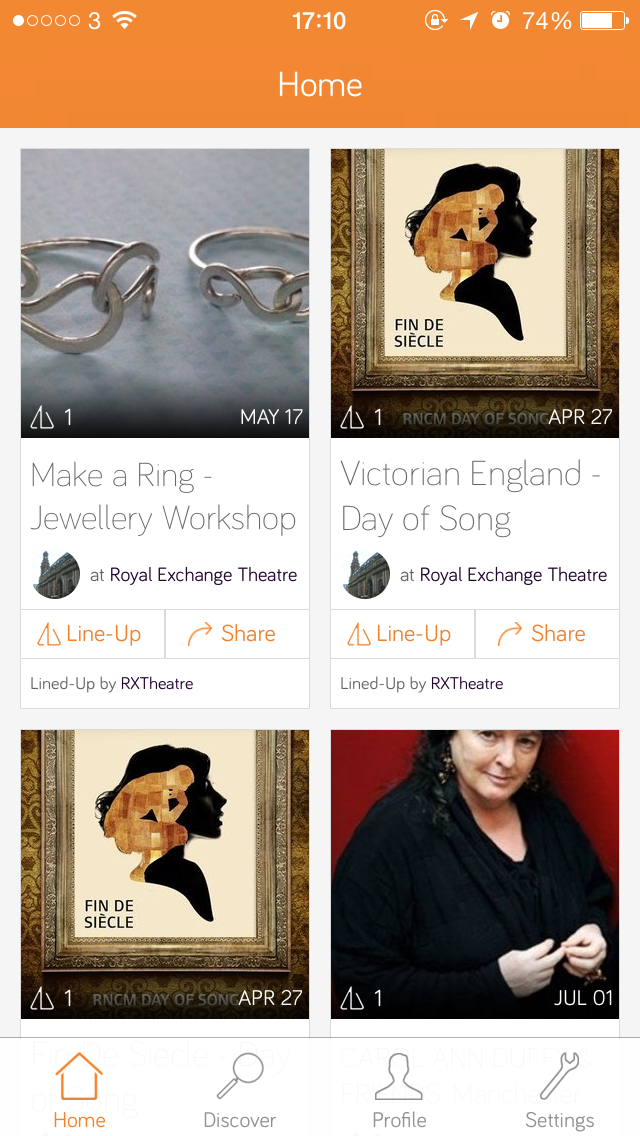
\includegraphics[width=0.3\textwidth]{Images/lineup}
				\label{fig:lineup}
			\end{figure}

		\subsubsection{Spotnight}
			Spotnight\cite{spotnight} shows selected events happening in the London area, it gives you the ability to purchase tickets for the events available through a 3rd party service. You can view the events that are happening either this week or later on, however you are able to apply filters for specific areas, style of music, and genres. The application allows you to like events, however this does not seem to have any particular effect to the ordering of the events or any other aesthetic/functional item of the application. When viewing an individual event, you are able to view the location, description, price, images, people attending, and venue contact details. You are also able to share particular events through social networking sites; Facebook and Twitter. 

			\begin{figure}[ht] % H - For exact position 
				\caption[Spotnight home screen]{Image showing the home screen for the Spotnight application }
				\centering
				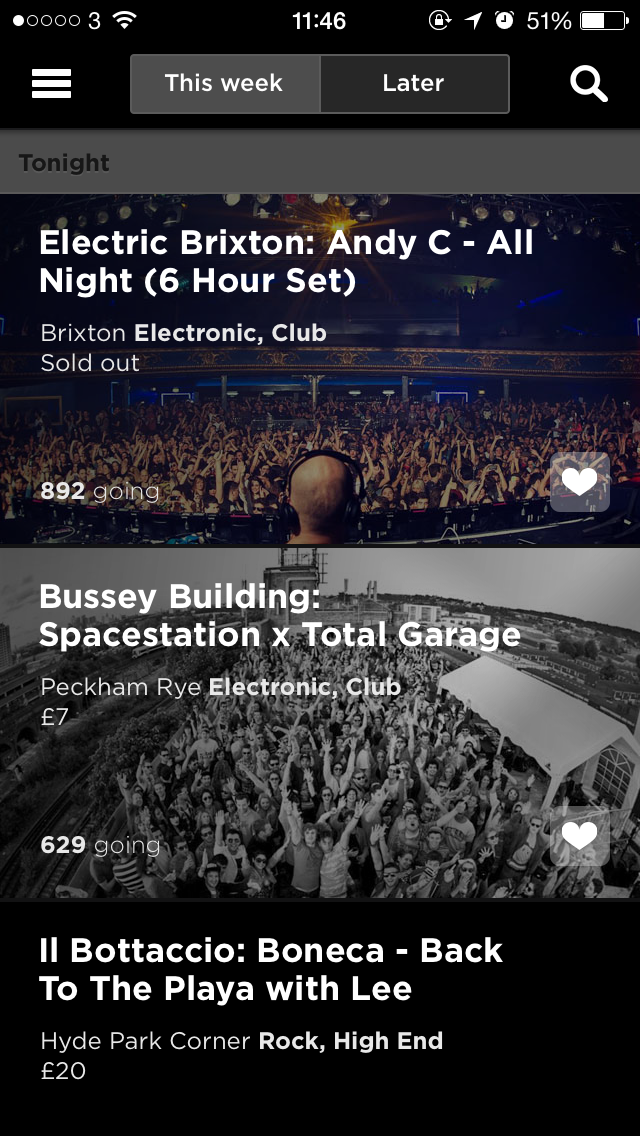
\includegraphics[width=0.3\textwidth]{Images/spotnight}
				\label{fig:spotnight}
			\end{figure}
		
		\subsubsection{Songkick}
			Songlick\cite{songkick} offers a selection of artist specific events, Songkick allows you to see events happening in your area, and by artist. From here you are presented with the details of the event including the line up, location and an option to purchase tickets via a 3rd party service. Songkick also allows you to track an event and mark an event as attending, to use these functions you are required to sign up however casual use of the application does not require signing up. The application also allows you to follow artists and will suggest events that are happening near you within the artists you are following.
			%  Add in screen shot of the application
			\begin{figure}[H] % H - For exact position 
				\caption[Songkick home screen]{Image showing the home screen for the Songkick application }
				\centering
				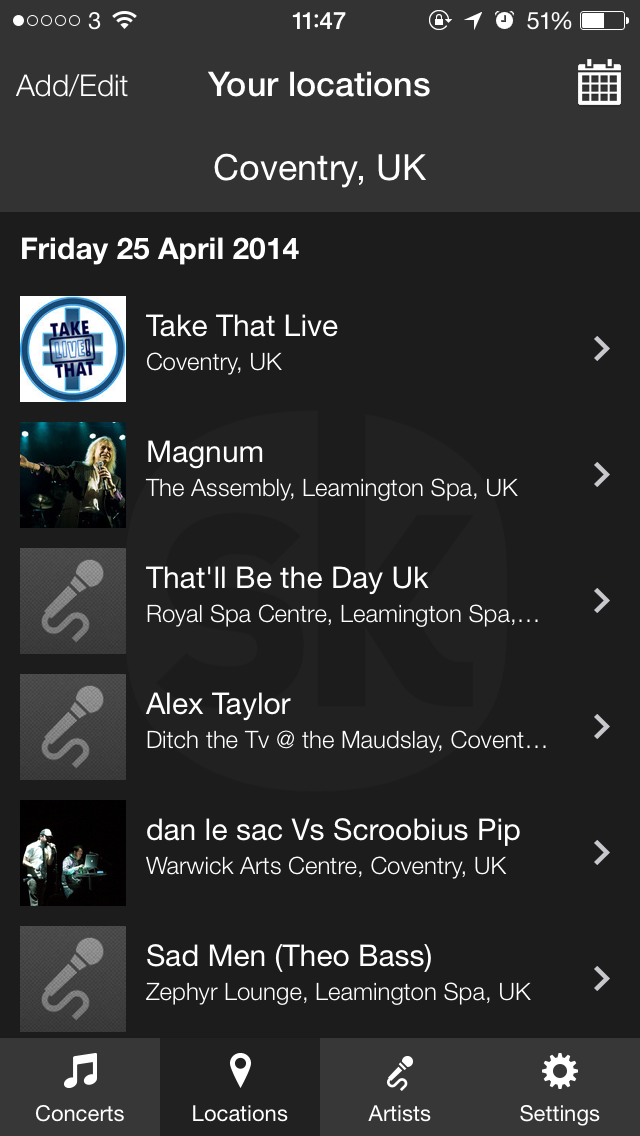
\includegraphics[width=0.3\textwidth]{Images/songkick}
				\label{fig:songkick}
			\end{figure}

\section{Analysis}

	With the main problem being users not knowing an area there is a prevalent set of key features that is required by the application for it to help solve the issue at hand. The most prominent being be able to grab the users current location and to be able to filter out the events that are happening near to their current location. However many people may not want to travel to the area only to find out that nothing that interests them is happening, so ideally the events should be categorised by area and then a user should be able to browse the areas they are visiting. Bearing this in mind, as the user is visiting a potentially new area they may require directions or some sort of map indicating the location of the event. 

	Another issue is that many of the previous systems require human interaction to find out about events and manually input these into to the system. Whilst this allows for a human based data validation it can be slow and time consuming to conduct, and result in only key events being selected and not provide a large enough range for their users. By use of data mining techniques we are able to pull in a must larger variety of events and therefore cater for a wider audience, thus allowing the user to actually discover new events that they may not have thought about. This relates to the first issue, by pulling in the details automatically from various API's we are able to half the work required by us and the promotions companies. Making the use of this service much more attractive to both parties, ultimately widening the stakeholders and potential audience. 		

	\subsection{Primary objectives}
		
		There a number of primary objectives for this task, these are listed below

		\begin{description}
			\item[Personalised feed] \hfill \\
				The application must produce a feed that's personalised to the currently logged in user
			\item[Registration/Authentication] \hfill \\
				The system must provide the ability to create a new user, and to login a previously registered user. They should also stay logged in until the have logged out of the account.
			\item[Ability to follow events] \hfill \\
				The application should provide functionality to follow an event to help facilitate the personalised feed. 
			\item[Categorise the events] \hfill \\
				The application should allow the events to be presented in multiple ways including categories and areas. 
			\item[Show individual events] \hfill \\
				The application must provide all of the relevant details of each event
			% \item[Directions to an event] \hfill \\
			% 	The application needs to be able to give a user either location information for the event or allow them to find directions from their current location. 
			\item[Connect to various API's] \hfill \\
				The server must be able to pull in information from a number of different API's and 
			\item[Application - Server interoperability] \hfill \\
				The application and server need to be able to pass information to each using some form of interoperability. 
		\end{description}

	\subsection{Secondary objectives}
		These objectives are not critical to the running of the application but provides extra functionality to the service. 

		\begin{description}
			\item[Location awareness] \hfill \\
				The application should be  of the location of the user, and only use the nearest events. 
			\item[Notifications] \hfill \\
				The user should receive notifications then events have been updated based off the data mining application.
			\item [User profile] \hfill \\
				The application should show a users profile, showing the events they are following and their personal details.
			\item[Link to purchase the events] \hfill \\
				The application should provide some sort of back link to enable a user to purchase tickets through a 3rd party service. 
		\end{description}

	\subsection{Hardware requirements}
		\begin{description}
			\item[Application must run on > iPhone 4] \hfill \\
				The iOS application must run on all iPhones that run the latest version of the iOS firmware.
			\item[Server should run on cloud computing provider] \hfill \\
				The server element should run on a cloud computer to allow for high demand with ease. 
		\end{description}

\section{iOS and Ruby on Rails}

	\subsection{iOS Development}
	The application itself will be based on the iOS platform for Apple iPhones, being programmed using Apples Objective C language. This decision was made based on some Google Analytics information, which was provided by a popular events company in Birmingham. Figure \ref{fig:googleAnalyticsRainbow} shows us the statistics that's been produced by Google Analytics showing that over 70\% of their traffic was coming from Apple iPhones. The programmer also had readily available access to an iPhone to assist with the development process underlined. 

	\begin{figure}[H] % H - For exact position 
		\caption[Image of Google Analytics for popular events site]{This image shows within a month their main traffic is through Apple iPhones, with secondary traffic of Android being a much smaller percentage. }
		\centering
		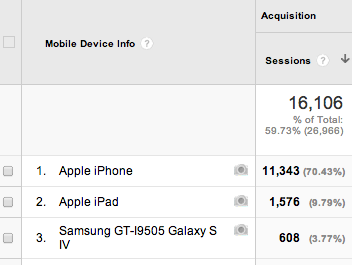
\includegraphics[scale=1]{Images/google-analytics}
		\label{fig:googleAnalyticsRainbow}
	\end{figure}

	To develop iOS applications you are required to use Apples own IDE XCode 5 packaged into this is the iOS simulator, this allows me to test applications developed locally on the machine without needing to make a payment to the developers network. The simulator allows for all parts of the application to be tested, however I will need to manually set up locations to test the location awareness of the application. I will also be utilising a package manager called CocoaPods \cite{cocoapods} which allows me to pull in various libraries with ease and make sure I'm using the latest versions with future updates. To get used to the new IDE and we will utilise the resources from Ray Wenderlichs sites\cite{raywender}, Ray gives many resources including sample projects that can be analysed and tutorials.  

	iOS has 2 main design patterns that are usually followed, the first being model view controller (MVC) this is implemented by having 3 main sections of code; a place where the data is defined/stored(model), a place where any business logic is performed(controller), and a place where the data is outputted(view). Typically you can find multiple instances of the MVC pattern inside of one project. However it also utilises a delegation \& target/action delegation is used to pass data between the multiple MVC's you will find inside a project, and target/action which is used by iOS to link buttons with methods to be called upon that button being selected.

	\subsection{Server Development}

	The project will also require a server side element to be able to mine the data and provide the data to the application, this will be written in Ruby using the Ruby on Rails framework. Using the framework gives access to lots of functionality not built into the core of Ruby and provides a production ready environment. Due to the explosive nature of applications, it's been decided to use cloud computing to be able to effectively manage the demand of resources used by the application. For this it was decided the best cloud platform is Heroku\cite{heroku} this was mainly due to the ease of deployment, which involved a git push to their remote server, and they provided a free tier during development. 

\section{Process}
	
	Mostly the methodology followed was a cut down version of agile, optimised for a single developer. This decision was made to allow the programmer to add in extra functionality as seen fit throughout the project, and to allow the design to flex with these requirements. To develop the bulk of the application feature driven development (FDD) was used as there were 3 main logical aspects to the project those being; Interoperability, iOS Application, and Data mining. Due to the nature of each of these sub sections, there will a slightly different sub-methodology for each. Each feature relies on one already being present bar the data mining feature, this is key to the order of features. The first feature developed was the data mining, which received information and input it into a database, the interoperability feature of the server element (REST API) and then the iOS application itself to use the server element of the project. Agile was also chosen as whilst we know the scope of the project currently, looking to the future it may be required to add in extra functionality based off the reception received. Inside of each feature was a set of iterations, these were primarily individual requirements for each feature. 

	\subsection{Server application}
		The development of the server application will be following the test driven development (TDD) methodology, utilising the red, green, re-factor ideology. This was chosen as it will allow for flexibility in the overall design of the application, and will also ensure tests are being written for the functionality of the software. By following TDD it will also ensure that the code is the most efficient, as no more code is written except for what's required to pass the various tests. 

	\subsection{iOS Application}
		The development of the iOS application was a lot more conventional, a feature was programmed with relevant unit testing implemented to ensure the functionality produced the correct output. A form of TDD was used as sometimes a test failed so it was required to go back and fix the code to ensure the test passed. After each feature was added, device testing was undertaken ensuring it all ties together well and works on the device.  
	